% !TEX program = pdflatex
%
% Artigo do Trabalho Final de PSI5120 (Topicos em Computacao em Nuvem).
% Template: IEEEtran (classe padrao, disponivel em qualquer distribuicao
% TeX Live/MiKTeX ou no Overleaf via "New Project > IEEE").
%
% ATENCAO (ver docs/ROTEIRO_EXECUCAO.md e docs/DECISIONS.md):
%   1. As figuras da Secao VI (Experimental Evaluation) so existem depois
%      de rodar scripts/load_test.py e scripts/analyze_results.py.
%      Rode o pipeline ANTES de compilar este PDF pela primeira vez.
%   2. Todo numero marcado com [PREENCHER] deve ser substituido pelo
%      valor real gerado em results/figures/resumo_estatistico.txt.
%   3. Troque o nome do autor abaixo (marcado com TODO) antes de entregar.

\documentclass[conference]{IEEEtran}
\usepackage{cite}
\usepackage{amsmath,amssymb,amsfonts}
\usepackage{graphicx}
\usepackage{textcomp}
\usepackage{xcolor}
\usepackage{booktabs}
\usepackage{url}
\usepackage{tikz}
\usetikzlibrary{shapes.geometric, arrows.meta, positioning}

\def\BibTeX{{\rm B\kern-.05em{\sc i\kern-.025em b}\kern-.08em
    T\kern-.1667em\lower.7ex\hbox{E}\kern-.125emX}}

\begin{document}

\title{Reliability and Observability Patterns for a Serverless Event-Driven Processing Pipeline on AWS: An Empirical Extension of a Lambda--SQS Architecture}

\author{
\IEEEauthorblockN{Pedro TODO-SOBRENOME}
\IEEEauthorblockA{Escola Politécnica, Universidade de São Paulo\\
PSI5120 --- Tópicos em Computação em Nuvem\\
São Paulo, Brazil\\
pedro.prda@gmail.com}
}

\maketitle

\begin{abstract}
Serverless event-driven architectures are widely promoted for their operational simplicity and pay-per-use cost model, yet introductory laboratory exercises typically demonstrate only the minimal mechanics of a function-as-a-service (FaaS) pipeline --- a trigger, a handler, and a dead-letter queue --- without the reliability and observability concerns that a production system must address. This paper describes an extension of a didactic AWS Lambda--SQS laboratory (Amazon Simple Queue Service with a dead-letter queue for controlled-failure demonstration) into a more complete event-processing pipeline: an HTTP ingestion layer built on Amazon API Gateway, idempotent persistence in Amazon DynamoDB to tolerate the at-least-once delivery semantics of SQS, and an observability layer combining Amazon CloudWatch alarms, custom metrics, and Amazon SNS notifications. The full infrastructure is provisioned as code with AWS CloudFormation. We evaluate the resulting pipeline experimentally under synthetic load, measuring request latency, success rate, dead-letter-queue redrive behavior, and idempotency correctness, and we discuss the trade-offs of this design relative to a container-orchestration alternative (Amazon EKS) explored earlier in the same course. Our results show [PREENCHER: resumo de 1 frase com p50/p95 e taxa de sucesso] and confirm that duplicate message deliveries are absorbed without double-processing side effects at the persistence layer.
\end{abstract}

\begin{IEEEkeywords}
cloud computing, serverless computing, AWS Lambda, Amazon SQS, event-driven architecture, reliability, observability, idempotency, infrastructure as code
\end{IEEEkeywords}

\section{Introduction}

Cloud computing has evolved from the utility-computing vision articulated by Buyya et al.~\cite{buyya2009}, centered on on-demand provisioning of virtualized infrastructure, toward increasingly managed abstractions in which the provider assumes responsibility not only for hardware but for the entire execution runtime. Function-as-a-Service (FaaS) platforms such as AWS Lambda represent the far end of this spectrum: developers submit application code and a trigger configuration, and the provider handles provisioning, scaling, and patching of the underlying compute. This shift changes what an engineer must reason about --- from capacity planning and virtual machine images, as in the private/hybrid IaaS clouds studied by Sotomayor et al.~\cite{sotomayor2009} and by the OpenNebula project~\cite{opennebula2011}, to message delivery semantics, retry policies, and the idempotency of individual event handlers.

This paper reports on an extension of a serverless laboratory exercise used in the PSI5120 course (Cloud Computing Topics) at Escola Politécnica, Universidade de São Paulo. The original exercise provisions a single AWS Lambda function triggered by an Amazon SQS queue, with a dead-letter queue (DLQ) to capture messages that fail repeatedly, and demonstrates this mechanism through a deliberately minimal handler that validates one numeric field and can be forced to fail on demand. While pedagogically effective for teaching the SQS--Lambda--DLQ retry mechanism in isolation, the exercise omits several concerns that any real deployment of this pattern must address: how events enter the system, how their processing results are persisted, how duplicate deliveries are handled, how operators are notified of failures, and how the system behaves under load.

We extend this laboratory along exactly these axes and treat the result as a small but complete case study in applying reliability engineering practices to a serverless pipeline. Concretely, our contributions are:

\begin{enumerate}
\item An HTTP ingestion layer (Amazon API Gateway, HTTP API) that decouples event producers from the processing pipeline, added in front of the original Lambda--SQS--DLQ mechanism without modifying its retry semantics.
\item An idempotent persistence layer (Amazon DynamoDB with a conditional write keyed on an application-level event identifier) that tolerates SQS's at-least-once delivery guarantee.
\item An observability layer combining a CloudWatch alarm on DLQ depth, an SNS email notification, and a custom CloudWatch metric, together with a CloudWatch dashboard.
\item An experimental evaluation under synthetic concurrent load, measuring latency distribution, success rate, and dead-letter-queue behavior, together with a qualitative cost comparison against a container-orchestration alternative.
\end{enumerate}

The remainder of this paper is organized as follows. Section~II reviews related work on cloud service models and infrastructure management. Section~III provides background on the specific AWS primitives used. Section~IV describes the extended system design. Section~V discusses implementation details. Section~VI presents the experimental evaluation. Section~VII discusses limitations and trade-offs. Section~VIII concludes.

\section{Related Work}

Buyya et al.~\cite{buyya2009} articulate an early and influential vision of cloud computing as a fifth utility, emphasizing on-demand provisioning, elasticity, and market-based resource allocation across IaaS, PaaS, and SaaS layers. Much of that vision --- particularly elasticity and pay-per-use billing --- is realized even more directly by FaaS platforms than by the IaaS model the paper primarily analyzes, since a Lambda function has no idle cost and requires no capacity planning at all; conversely, aspects of the original vision built around SLA-driven markets for virtual machine capacity have limited applicability once the unit of billing becomes a single function invocation measured in milliseconds.

Sotomayor et al.~\cite{sotomayor2009} describe virtual infrastructure management for private and hybrid clouds, focusing on the OpenNebula system's ability to orchestrate virtual machines across local and remote (public cloud) resources. This work, and the OpenNebula project more broadly~\cite{opennebula2011}, represents the IaaS/virtualization layer of cloud infrastructure --- the same conceptual layer exercised in the private-cloud laboratory earlier in the PSI5120 course. Our work sits one abstraction level above: rather than managing virtual machine placement, we manage the composition and reliability behavior of managed serverless services, where the underlying compute placement is entirely opaque to the application developer. Section~VII returns to this contrast explicitly, comparing the serverless design studied here with the managed-Kubernetes (Amazon EKS) laboratory from the same course.

Beyond the three works used as required reading in the course, our extension draws directly on AWS's own architectural guidance for decoupled, queue-based processing and on the well-documented semantics of Amazon SQS (at-least-once delivery, visibility timeout, and redrive policies) and AWS Lambda (event source mappings, concurrency, and execution roles), which we summarize in Section~III for readers unfamiliar with these specific primitives.

\section{Background}

\subsection{Amazon SQS delivery semantics}
Amazon SQS is a managed message queue that guarantees at-least-once delivery: a message may be delivered to a consumer more than once, for example if the consumer fails to delete it within the queue's \emph{visibility timeout}. A \emph{redrive policy} can be attached to a queue specifying a \emph{dead-letter queue} (DLQ) and a \emph{maxReceiveCount}; after a message has been received (and not deleted) that many times, SQS automatically moves it to the DLQ instead of redelivering it. This is the mechanism the original PSI5120 Lab 07 exercise demonstrates directly.

\subsection{AWS Lambda event source mappings}
An AWS Lambda \emph{event source mapping} polls a queue and invokes a function with a batch of messages. When a function invocation raises an exception, SQS treats the messages in that batch as not deleted (with \emph{BatchSize}=1, exactly one message), so they become eligible for redelivery according to the visibility timeout, eventually triggering the redrive policy above.

\subsection{Idempotency under at-least-once delivery}
Because SQS delivery is at-least-once rather than exactly-once, any handler with externally visible side effects (such as writing a database record) must be written to tolerate duplicate invocations for the same logical event. A common pattern, used in this work, is to derive an idempotency key from the event payload and perform a \emph{conditional write} to a key-value store that fails if the key already exists, allowing the handler to detect and skip duplicate processing.

\subsection{Managed observability primitives}
Amazon CloudWatch collects metrics (built-in, such as queue depth, and custom, published by application code) and supports alarms that transition state based on a metric threshold. Amazon SNS is a managed publish-subscribe service that can deliver an alarm state transition to a human operator (for example, by email) or to another system.

\section{System Design}

Fig.~\ref{fig:architecture} shows the extended architecture. The shaded components (SQS main queue, DLQ, and the consumer Lambda's core validation logic) are inherited unchanged from the original Lab 07 exercise; the remaining components are the extension described in this paper.

\begin{figure}[htbp]
\centering
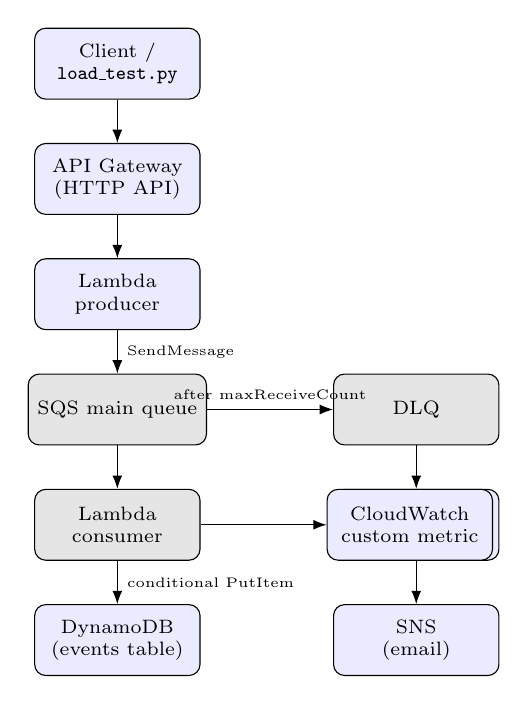
\begin{tikzpicture}[
    node distance=0.55cm and 0.9cm,
    box/.style={draw, rounded corners, align=center, minimum height=0.9cm, minimum width=2.1cm, font=\scriptsize},
    inherited/.style={box, fill=gray!20},
    added/.style={box, fill=blue!8},
    arr/.style={-Latex, thin}
]
\node[added] (client) {Client /\\ \texttt{load\_test.py}};
\node[added, below=of client] (api) {API Gateway\\(HTTP API)};
\node[added, below=of api] (producer) {Lambda\\producer};
\node[inherited, below=of producer] (queue) {SQS main queue};
\node[inherited, below=of queue] (consumer) {Lambda\\consumer};
\node[added, below=of consumer] (ddb) {DynamoDB\\(events table)};

\node[inherited, right=1.6cm of queue] (dlq) {DLQ};
\node[added, below=of dlq] (alarm) {CloudWatch\\alarm};
\node[added, below=of alarm] (sns) {SNS\\(email)};
\node[added, right=1.6cm of consumer] (cw) {CloudWatch\\custom metric};

\draw[arr] (client) -- (api);
\draw[arr] (api) -- (producer);
\draw[arr] (producer) -- node[right, font=\tiny]{SendMessage} (queue);
\draw[arr] (queue) -- (consumer);
\draw[arr] (consumer) -- node[right, font=\tiny]{conditional PutItem} (ddb);
\draw[arr] (queue.east) -- node[above, font=\tiny]{after maxReceiveCount} (dlq.west);
\draw[arr] (dlq) -- (alarm);
\draw[arr] (alarm) -- (sns);
\draw[arr] (consumer.east) -- (cw.west);
\end{tikzpicture}
\caption{Extended pipeline architecture. Gray boxes are inherited from the original PSI5120 Lab~07 exercise; blue boxes are added by this work.}
\label{fig:architecture}
\end{figure}

Table~\ref{tab:extension} summarizes the gap between the original laboratory and this work, and maps each addition to the AWS service used to close it.

\begin{table}[htbp]
\caption{Extension summary}
\label{tab:extension}
\centering
\begin{tabular}{p{2.6cm}p{2.6cm}p{2.2cm}}
\toprule
\textbf{Gap in Lab 07} & \textbf{Extension} & \textbf{AWS service} \\
\midrule
No ingestion endpoint & Decoupled HTTP entry point & API Gateway \\
No persistence & Store processed event outcome & DynamoDB \\
No duplicate handling & Conditional write keyed on \texttt{event\_id} & DynamoDB \\
No operator alerting & Alarm on DLQ depth & CloudWatch + SNS \\
No quantitative evaluation & Load test with latency/throughput measurement & --- (custom script) \\
\bottomrule
\end{tabular}
\end{table}

The design deliberately preserves the original queue configuration inherited from Lab~07 (30-second visibility timeout, \texttt{maxReceiveCount}=2, \texttt{BatchSize}=1) so that the retry-to-DLQ behavior being taught in the original exercise remains observable and comparable in the extended system.

\section{Implementation}

The entire infrastructure is defined in a single AWS CloudFormation template (\texttt{infra/template.yaml}), extending the template distributed with the original laboratory. Both Lambda functions are implemented in Python 3.12 and are embedded directly in the template (matching the deployment pattern of the original exercise) to avoid requiring a separate artifact build/upload step, at the cost of manually keeping the embedded code synchronized with the human-readable copies kept under \texttt{src/} for local reading and testing --- a trade-off discussed further in Section~VII.

\subsection{Producer function}
The producer function is invoked synchronously by API Gateway using the Lambda proxy integration (payload format version 2.0). It parses and minimally validates the JSON request body, assigns a UUID \texttt{event\_id} when the caller does not supply one, and publishes the payload unchanged to the SQS main queue via \texttt{sqs:SendMessage}. It returns HTTP~202 (Accepted) with the assigned \texttt{event\_id}, signalling that processing is asynchronous.

\subsection{Consumer function}
The consumer function is the direct descendant of the original Lab~07 handler: the event-normalization logic (handling both direct invocation and the single-record SQS batch format) and the controlled-failure branch (\texttt{forcar\_falha}) are unchanged. Two behaviors were added at the end of the handler: (i) a conditional \texttt{PutItem} to the DynamoDB \texttt{events} table with \texttt{ConditionExpression=attribute\_not\_exists(event\_id)}, which fails with \texttt{ConditionalCheckFailedException} when the same \texttt{event\_id} has already been recorded, allowing the handler to distinguish a first-time write from a duplicate delivery; and (ii) a custom CloudWatch metric (\texttt{EventosProcessados}, namespace \texttt{PSI5120/TrabalhoFinal}) dimensioned by event type and outcome, feeding the dashboard described below.

\subsection{Observability}
A CloudWatch alarm monitors \texttt{ApproximateNumberOfMessagesVisible} on the DLQ (threshold~$\geq 1$, one 60-second evaluation period) and publishes state transitions to an SNS topic with an email subscription. A CloudWatch dashboard aggregates Lambda invocation/error counts for both functions, queue depth for the main queue and the DLQ, and the custom metric described above.

\subsection{Infrastructure as code and least privilege}
Each Lambda function has its own IAM execution role, scoped to only the actions it needs (the producer role can only send messages to the main queue and write its own log group; the consumer role can additionally receive/delete from the main queue, write to the DynamoDB table, and publish CloudWatch metrics). The \texttt{cloudwatch:PutMetricData} action does not support resource-level restriction in IAM and therefore necessarily uses a wildcard resource, a documented and accepted limitation of the AWS permission model rather than a design choice of this project.

\section{Experimental Evaluation}

\subsection{Methodology}
We used the load-generation script \texttt{scripts/load\_test.py} to issue $N$ concurrent HTTP POST requests against the API Gateway endpoint, with a configurable fraction $f$ of requests carrying \texttt{forcar\_falha=true} to exercise the DLQ path. Each request's end-to-end latency (from request submission to receipt of the HTTP~202 response) was recorded client-side. Results were analyzed with \texttt{scripts/analyze\_results.py}.

\emph{[PREENCHER: descreva aqui os parâmetros reais usados, ex.: ``We ran $N=150$ requests with concurrency 15 and $f=0.10$ from a single client machine on residential broadband in Region X against the \texttt{us-east-1} deployment.'']}

\subsection{Latency and throughput}
Fig.~\ref{fig:latency-hist} and Fig.~\ref{fig:latency-series} show the distribution and time series of end-to-end request latency. \emph{[PREENCHER: p50 = XX ms, p95 = XX ms, p99 = XX ms, taxa de sucesso = XX\%, conforme results/figures/resumo\_estatistico.txt]}.

\begin{figure}[htbp]
\centering
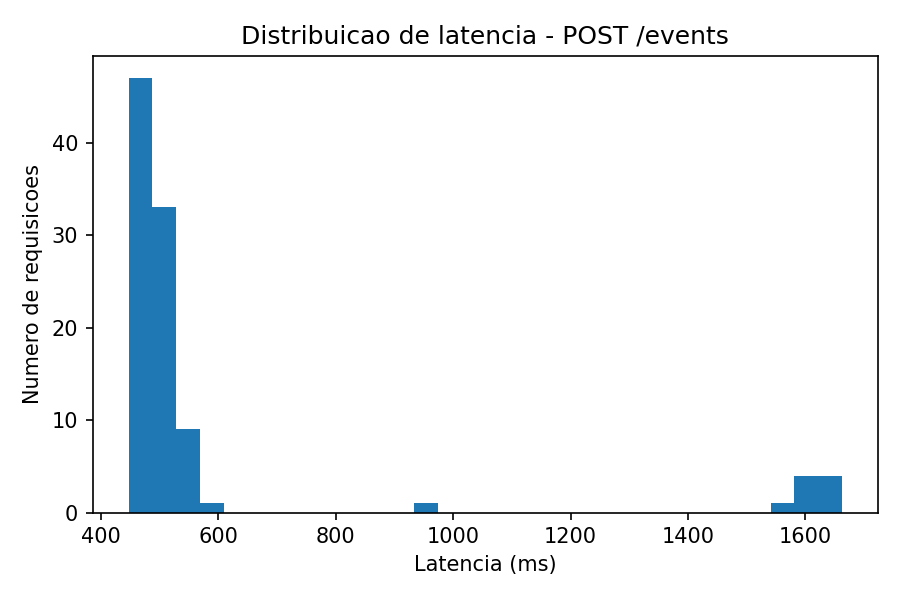
\includegraphics[width=0.95\linewidth]{../results/figures/latencia_histograma.png}
\caption{Distribution of end-to-end request latency.}
\label{fig:latency-hist}
\end{figure}

\begin{figure}[htbp]
\centering
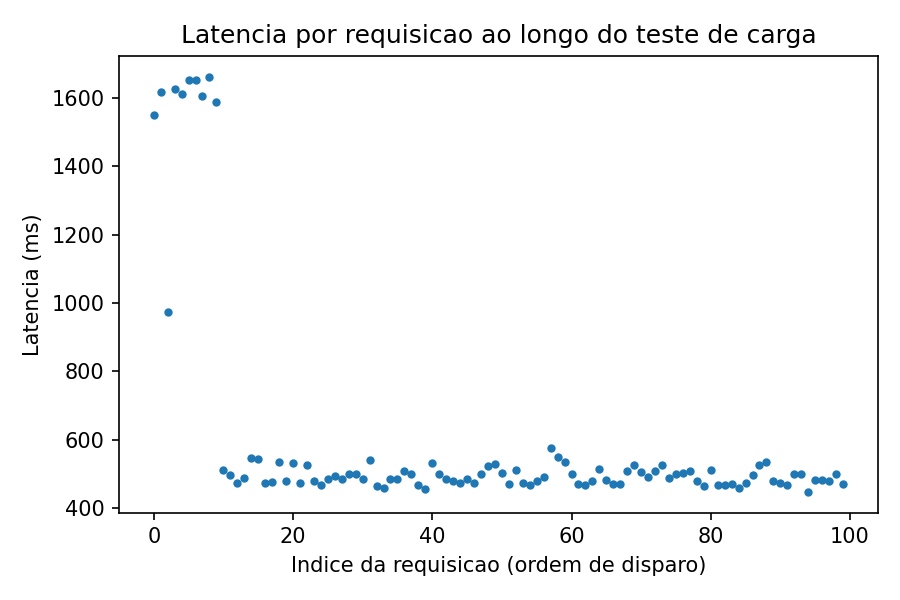
\includegraphics[width=0.95\linewidth]{../results/figures/latencia_serie.png}
\caption{Request latency over the course of the load test.}
\label{fig:latency-series}
\end{figure}

\subsection{Failure handling and dead-letter behavior}
Fig.~\ref{fig:success-rate} compares the HTTP acceptance rate between normal events and events marked with \texttt{forcar\_falha}. Because the producer function only validates and enqueues the request, both classes of event are accepted at the API layer; the difference in outcome is only observable downstream, in the DLQ depth and in the CloudWatch Logs of the consumer function. \emph{[PREENCHER: número de mensagens que chegaram à DLQ durante o teste, tempo até a primeira mensagem aparecer na DLQ, e se o alarme/e-mail disparou corretamente.]}

\begin{figure}[htbp]
\centering
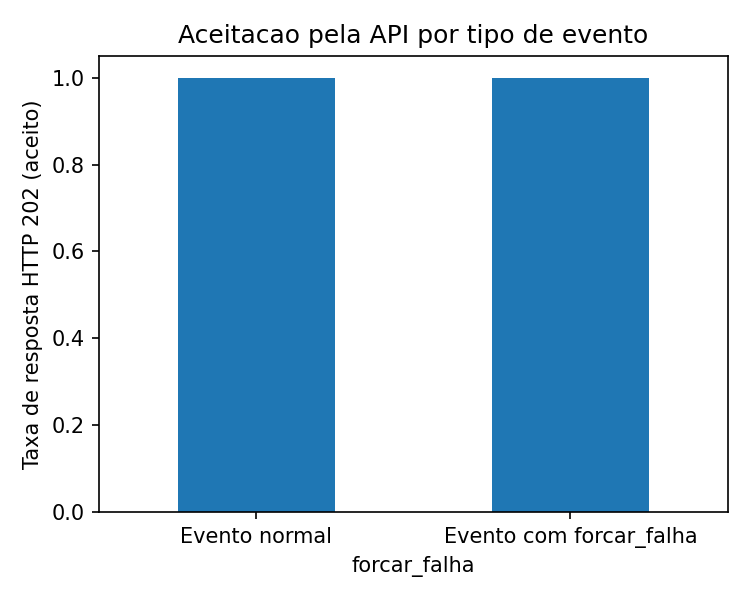
\includegraphics[width=0.8\linewidth]{../results/figures/taxa_sucesso.png}
\caption{API acceptance rate by event type.}
\label{fig:success-rate}
\end{figure}

\subsection{Idempotency correctness}
We manually issued two identical requests sharing the same \texttt{event\_id}, as described in \texttt{docs/ROTEIRO\_EXECUCAO.md} (Section~4.3). \emph{[PREENCHER: confirme que apenas um item foi persistido no DynamoDB e cole o trecho de log com "fase": "duplicata\_idempotente".]}

\subsection{Cost}
Because both Lambda functions run in well under a second per invocation and all other services used (API Gateway HTTP API, SQS, DynamoDB on-demand, CloudWatch, SNS) bill per request/GB with a free tier, the workload evaluated here remained within AWS's free-tier allowances. \emph{[PREENCHER: se desejar, inclua uma estimativa de custo mensal para um volume de produção hipotético, comparando com os preços de EC2/EKS/Load Balancer já levantados na Aula 06 (ver Aula 06/Prática/evidencias/E8\_precos-*.png), e cite a fonte dos preços com data de consulta.]}

\section{Discussion}

\subsection{Idempotency of effects versus idempotency of execution}
The idempotency mechanism implemented here guarantees that the \emph{persisted effect} of a duplicate delivery is idempotent (at most one row is ever written per \texttt{event\_id}), but it does not prevent the \emph{business logic itself} from executing twice, since the conditional write happens after validation rather than before it. This is an acceptable trade-off for a handler with no externally visible side effects beyond the database write, but it would not be sufficient for a handler that, for example, calls a non-idempotent third-party payment API; a stricter \emph{reserve-then-process} pattern (writing a placeholder row before executing business logic) would be required in that case.

\subsection{Serverless versus managed Kubernetes}
The same course includes a laboratory provisioning an Amazon EKS cluster for a comparable workload (Section~VI of the Aula~06 materials measured indicative hourly prices for EC2 worker nodes, the EKS control plane, and an Application Load Balancer). Unlike that architecture, the pipeline described here has no idle cost and no cluster lifecycle to manage (cluster creation/deletion on EKS took on the order of 15--20 minutes each in that exercise, against roughly one to three minutes to deploy or tear down the CloudFormation stack used here). The trade-off is reduced control over the execution environment and per-invocation cold-start latency, which is outside the scope of the load test performed here but is a well-documented characteristic of FaaS platforms.

\subsection{Operational simplicity versus code duplication}
Embedding the Lambda source code directly in the CloudFormation template, following the pattern of the original laboratory, avoids requiring an S3 deployment bucket or a packaging tool, which matters for an audience with no prior AWS experience (see \texttt{docs/ROTEIRO\_EXECUCAO.md}). The cost of this choice is that the human-readable copies of the same code kept under \texttt{src/} must be kept manually synchronized with the copies embedded in the template; for a larger project this would be resolved with a packaging pipeline (for example, the AWS SAM CLI), which we deliberately avoided here to keep the number of prerequisite tools low.

\subsection{Threats to validity}
The load test was executed from a single client process against a single AWS region, which measures end-to-end latency as experienced from one network vantage point rather than the server-side processing latency alone; it therefore reflects a combination of network conditions and pipeline behavior. \emph{[PREENCHER: comente aqui qualquer limitação observada durante a execução real do teste, por exemplo throttling, variação de latência entre rodadas, etc.]}

\section{Conclusion and Future Work}

We extended a didactic AWS Lambda--SQS laboratory exercise into a more complete serverless event-processing pipeline, adding an HTTP ingestion layer, idempotent persistence, and an observability layer, while preserving the retry-to-dead-letter-queue mechanism taught in the original exercise. The resulting system was evaluated experimentally under synthetic concurrent load. \emph{[PREENCHER: uma frase final resumindo os principais números observados.]} Future work could extend the idempotency mechanism to a reserve-then-process pattern for handlers with non-idempotent side effects, replace the manually synchronized inline Lambda code with a packaging pipeline, and add AWS X-Ray tracing to attribute latency across the producer, queue, and consumer stages individually rather than only end-to-end.

\section*{Acknowledgment}
This work extends laboratory material developed for the PSI5120 course at Escola Politécnica, Universidade de São Paulo.

\begin{thebibliography}{00}

\bibitem{buyya2009}
R. Buyya, C. S. Yeo, S. Venugopal, J. Broberg, and I. Brandic, ``Cloud computing and emerging IT platforms: Vision, hype, and reality for delivering computing as the 5th utility,'' \emph{Future Generation Computer Systems}, vol. 25, no. 6, pp. 599--616, 2009.

\bibitem{sotomayor2009}
B. Sotomayor, R. S. Montero, I. M. Llorente, and I. Foster, ``Virtual infrastructure management in private and hybrid clouds,'' \emph{IEEE Internet Computing}, vol. 13, no. 5, pp. 14--22, Sept./Oct. 2009.

\bibitem{opennebula2011}
D. Milojičić, I. M. Llorente, and R. S. Montero, ``OpenNebula: A cloud management tool,'' \emph{IEEE Internet Computing}, vol. 15, no. 2, pp. 11--14, Mar./Apr. 2011.

\end{thebibliography}

\end{document}
